% vim: set tw=78 sts=2 sw=2 ts=8 aw et ai:
\documentclass{workshop}

% Comentează liniile de mai jos în cazul în care nu există cod de inclus.
\usepackage{code/highlight}
\usepackage{color}        % dacă e folosit highlight
\usepackage{alltt}        % dacă e folosit highlight
\usepackage{amsfonts} 

\title[Sesssion 9]{Session 9}
\subtitle{Linux in Embedded Systems}
\author{Andrei Voinescu}
\date{12th July, 2012}

\begin{document}

% Arătăm numărul frame-ului
\setbeamertemplate{footline}[frame number]

\frame{\titlepage}

% NB: Secțiunile nu sunt marcate vizual, ci doar apar în cuprins
\section{Introduction}

\subsection{}

\begin{frame}{Introduction}
What we will be covering today
\begin{itemize}
	\item Why we use Linux in Embedded Systems
	\item How a Linux-capable board looks like
	\item How a Linux system boots up	
\end{itemize}
\visible<2->{What we will NOT be covering
\begin{itemize}
	\item How to develop Linux applications
	\item How to debug a module remotely via ssh
	
\end{itemize}
}
\visible<3->{What we will experiment
\begin{itemize}
\item How to write a simple device driver for an embedded board
\end{itemize}
}
\end{frame}

\begin{frame}{Linux in the Embedded World}
\begin{itemize}
\item Linux exists in many embedded devices
	\begin{itemize}
		\item Routers, NASs, Displays
		\item Smartphones, tablets, ebook-readers
	\end{itemize}

\visible<2->{
\item .. But Why?
	\visible<3->{
	\begin{itemize}
		\item Linux kernel offers drivers for many commonly used components
		\item Complete networking stacks
		\visible<4->{
		\item Linux system offers many utilities and libraries
			\begin{itemize}
				\item coreutils
				\item SSH, http servers, mysql,...
			\end{itemize}

		\visible<5->{
		\item Many hypervisors already support Linux as a guest system
		}
		}
	\end{itemize}
}
}
\end{itemize}
\end{frame}

\section{Example of a Linux System}
\begin{frame}{ATNGW100}
\only<1>{
\begin{figure}
	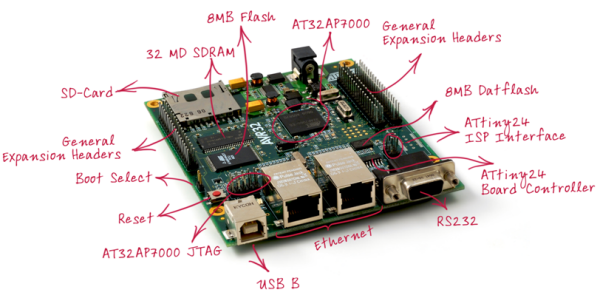
\includegraphics[width=1\textwidth]{img/Ngwoverview.png}
\end{figure}
}
\only<2>{
Key features:
\begin{itemize}
	\item 140MHz processor (AT32AP7000)
	\item 32MB SDRAM
	\item 8MB Parallel Flash
	\item 8MB Serial Flash
	\item 2x Ethernet ports
	\item USB B port (device port)
	\item RS232
\end{itemize}
}
\end{frame}

\begin{frame}{Linux prerequisites}
\begin{itemize}
		\definecolor{darkgreen}{RGB}{0,100,0}
	\item 32-bit processor \visible<2-> {\textcolor{darkgreen}{\checkmark}}
	\visible<3->{\item MMU} \visible<4-> {\textcolor{darkgreen}{AP7000 is a SoC with many peripherals, and a MMU \checkmark}}
	\visible<5->{\item  Location to run bootloader from } 
		\visible<6-> {\textcolor{darkgreen}{Bootloader is in Parallel Flash \checkmark}}
\end{itemize}
\end{frame}

\begin{frame}{Linux components}
	\begin{itemize}
		\visible<1-> {\item The Kernel}
		\visible<2-> {\item Filesystem
			\begin{itemize}
				\item Coreutils
				\item Userspace Applications
			\end{itemize}
		}
	\end{itemize}
	\visible<3-> { How can we compile these?}

	\visible<4->{
		\begin{itemize}
			\item Gcc
			\visible<5->{
				\begin{itemize}
					\item Which GCC?
				\end{itemize}
			}
		\end{itemize}
	}
	\visible<6->{
		Luckily, build systems exist...
		\begin{itemize}
			\item Buildroot
			\item Bitbake
			\item Yocto Project
		\end{itemize}
	}
\end{frame}

\section{Booting Up}
\subsection{}
\begin{frame}{Bootloaders}
	\begin{itemize}
		\item Processors always start execution at a specific address
		\item The code there loads the boot image of ("bootloader")
			\begin{itemize}
				\item Linux
				\item Other OS, maybe RT OS
				\item Application
			\end{itemize}

		\item In the case of Linux
			\begin{itemize}
				\item It loads the image into memory, it can load it from multiple locations (U-Boot supports MMC, TFTP, Flash, etc.)
				\item It gives the command line for the linux kernel (most importantly, the console and the root filesystem location)
				\item Many bootloaders offer limited scripting 
			\end{itemize}
	\end{itemize}
\end{frame}

\begin{frame}{Bootloader loading kernel image}
\input{code/start.tex}
\end{frame}

\begin{frame}{Kernel Initialization}
\only<1>{
\begin{itemize}
	\item The kernel needs to uncompress itself first\\
	\item CPU initialization
		\begin{itemize}
			\item Identify CPU
			\item Identify MMU setting
			\item Initialize MMU, flush TLB
		\end{itemize}
	\item Board initialization
		\begin{itemize}
			\item Serial line, \texttt{ttyS0}
			\item Initialize Parallel Flash, \texttt{physmap-flash.0}
			\item Initialize SPI Link
				\begin{itemize}
					\item Find SPI Dataflash (8MB)
				\end{itemize}
			\item Initialize MAC chips through MII (Media Independent Interface)
		\end{itemize}
\end{itemize}
}
\only<2>{
	\input{code/kernel.tex}
}
\only<3>{
	\input{code/board.tex}
}
\only<4>{
	\begin{itemize}
		\item Final step is to mount root
			\begin{itemize}
				\item Request DHCP... again
				\item Connect to portmapper running on server
				\item Find nfs and mountd ports from portmapper
			\end{itemize}
	\end{itemize}
	\input{code/nfs.tex}
}
\end{frame}

\begin{frame}{System Initialization}
\begin{itemize}
	\item Init process
		\begin{itemize}
			\item Spawns shells or logins
			\item Runs init scripts according to runlevel\\
				\vskip5pt
				\begin{tabular}{cl}
					\hline
					\textbf{Runlevel} & \textbf{Mode} \\
					\hline
					0 & System shutdown \\
					1 & Single user mode \\
					3 & Multiuser mode \\
					5 & Multiuser mode with X\\
					6 & System reboot \\
					\hline
				\end{tabular}
				\vskip5pt
		\end{itemize}
	\item Scripts reside in \texttt{/etc/init.d} directory
	\item Symlinks to scripts are in \texttt{/etc/rc}\textit{N}\texttt{.d}
\end{itemize}
\end{frame}

\section{Practical}
\subsection{}
\begin{frame}{LED. The module.}
	\begin{itemize}
		\item Default driver has sysfs interface
			\begin{itemize}
				\item \texttt{/etc/sys/class/leds}
			\end{itemize}
		\item Pins are grouped in 32-pin ports
		\item Each port has 4 important registers to control data output
			\begin{itemize}
				\item \texttt{PER} - Pin enable register
				\item \texttt{OER} - Output enable register
				\item \texttt{CODR} - Clear output data register
				\item \texttt{SODR} - Set output data register
			\end{itemize}
		\item Each register has 32bits, corresponding to pins (pin 0 is MSb)
		\item To set a pin to 0, we must
			\begin{itemize}
				\item Enable the pin (bit in \texttt{PER})
				\item Enable output on the pin (bit in \texttt{OER})
				\item Clear the value (set 1 in the bit in \texttt{CODR})
			\end{itemize}
	\end{itemize}
\end{frame}

\end{document}
